\probbatch{2}
\probno{7}
\probname{čočkování}
\proborigin{Karel vykradl katedru didaktiky fyziky.}
\probpoints{8}
\probsolauthors{pikalek}
\probsolvers{65}
\probavg{5,46}
\probtask{%
V~obálce jste spolu se zadáním dostali i~dvě čočky. Vaším úkolem je změřit jejich 
parametry~–~druh a~ohniskovou vzdálenost.\\
\ifyearbook
\else
\emph{Poznámka}\quad Pokud nejste stávající řešitelé FYKOSu, ale máte zájem se jimi stát, 
pak neváhejte a~objednejte si čočky až domů. A~to s~dostatečným předstihem, aby vám 
stihly dojít včas. Objednávejte na emailu \mail{cocky@fykos.cz}.
\fi
}
\makeatletter % na takové zanoření to (zatím) není děláno...
 \providecommand\subsubsubsection{\@startsection{paragraph}{4}{\z@}%
  {-2.25ex \@plus -1ex \@minus -.2ex}%
  {0.75ex \@plus.2ex}%
  {\normalfont\sffamily\slshape\small}}
\makeatother
\probsolution{%
Každý řešitel obdržel pro změření jinou dvojici čoček, naměřené hodnoty tedy
nebudou v~tomto řešení uvedeným hodnotám odpovídat.

V~této úloze budeme uvažovat pouze tenké čočky, tedy takové čočky, jejichž
tloušťka je malá oproti křivosti lámavých ploch. Navíc zanedbáme vady čoček
(chromatickou vadu, sférické zkreslení, koma).

\subsubsection{Druhy čoček}

Existují dva druhy kulových čoček -- spojky a~rozptylky. Odlišit je od sebe na
první pohled je jednoduché, spojky jsou ve středu tlustší než na kraji,
rozptylky právě naopak. Další odlišnost získáme pohledem skrz čočku na blízký
předmět. V~případě spojky bude předmět zvětšen (spojky se používají jako lupy),
skrz rozptylku uvidíme předmět naopak zmenšený. Třetí, na první pohled viditelný
rozdíl, je v~orientaci obrazu. Podíváme-li se skrz spojku na vzdálený předmět
tak, abychom jej viděli ostře, budeme předmět vidět převrácený (a~zmenšený),
zatímco u~rozptylky bude přímý (a~též zmenšený).

Čočky dále diferencujeme podle jejich tvaru, viz tabulka~\ref{R25S2U7_typy_cocek}.

\begin{table}[h!]
    \centering
    \ifyearbook\footnotesize\else\relax\fi
    \caption{Rozdělení čoček podle tvaru}
    \label{R25S2U7_typy_cocek}
    \begin{tabular}{cl@{\hspace{0.6cm}}@{\hspace{0.6cm}}cl}
        \multicolumn{2}{c@{\hspace{0.9cm}}}{\textbf{Spojky}}    &    \multicolumn{2}{c}{\textbf{Rozptylky}}    \\\\
        \multirow{2}{*}{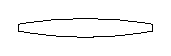
\includegraphics{problem2-7-typy-cocek11.eps}}    &    dvojvypuklá    &
        \multirow{2}{*}{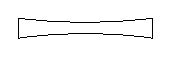
\includegraphics{problem2-7-typy-cocek21.eps}}    &    dvojdutá    \\
        & (bikonvexní) & & (bikonkávní) \\\\
        \multirow{2}{*}{
\includegraphics{problem2-7-typy-cocek12.eps}}    &    ploskovypuklá    &
        \multirow{2}{*}{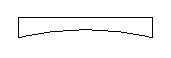
\includegraphics{problem2-7-typy-cocek22.eps}}    &    ploskodutá    \\
        & (plankonvexní) & & (plankonkávní) \\\\
        \multirow{2}{*}{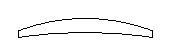
\includegraphics{problem2-7-typy-cocek13.eps}}    &    dutovypuklá    &
        \multirow{2}{*}{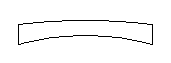
\includegraphics{problem2-7-typy-cocek23.eps}}    &    vypuklodutá    \\
        & (konkávkonvexní) & & (konvexkonkávní)
    \end{tabular}
\end{table}

Kromě kulových čoček existují i~jiné druhy: asférické čočky (používané
třeba v~objektivech fotoaparátů), Fresnelovy čočky (najdeme je třeba v~reflektorech,
zpětných projektorech, na majácích apod.) atd. Těmi se však dále nebudeme
zabývat.

\subsubsection{Výpočet ohniskové vzdálenosti z~poloměrů křivosti}

Podaří-li se nám změřit poloměry křivosti $ R_1 $ a~$ R_2 $ obou ploch
čočky (pro rovné plochy čoček je střed křivosti v~nekonečnu, tedy např. $
{1}/{R_1} = 0 $) a~víme-li, z~jakého materiálu je daná čočka vyrobena (známe
tedy index lomu $ n $ tohoto materiálu), můžeme ohniskovou vzdálenost~$ f $
(resp.optickou mohutnost~$ D $) této čočky spočítat ze vztahu
\eq{
    D = \frac{1}{f} = \left( n - 1 \right) \left( \frac{1}{R_2} - \frac{1}{R_1} \right) \,.
}

\ifyearbook%
\illfig{problem2-7-vypocet-polomeru.eps}{Výpočet poloměru křivosti}{R25S2U7_vypocet_polomeru}{7}%
\else%
\illfig{problem2-7-vypocet-polomeru.eps}{Výpočet poloměru křivosti}{R25S2U7_vypocet_polomeru}{5}%
\fi

Zjistit poloměry křivosti je možné přímo u~vypuklých ploch čoček. Upevníme čočku
kolmo nad milimetrový papír a~čočku z~větší vzdálenosti (kvůli omezení vlivu
perspektivy) takto kolmo na milimetrový papír vyfotíme. Na fotografii 
určíme výšku $ v $ a~délku tětivy $ l $
(viz obrázek~\ref{R25S2U7_vypocet_polomeru}) a~poloměr plochy spočítáme jako 
\eq{
    r = \frac{v^2 + \frac{t^2}{4}}{2 v} \,.
}

Je zřejmé, že tuto metodu můžeme použít pouze u~vypuklých ploch čoček. U~dutých
zakřivených ploch budeme muset použít složitější metodu měření. Využijeme toho,
že část světla se na této ploše odráží, a~ta se tak chová jako duté zrcadlo.
Umístíme-li před takovouto čočku předmět, vznikne na téže straně čočky skutečný
(tedy převrácený) obraz tohoto předmětu. Ze vzdálenosti předmětu a~obrazu od
zrcadla dokážeme určit jeho ohniskovou vzdálenost, a~tedy i~poloměr křivosti.

Nicméně stále neznáme index lomu materiálu, ze kterého je čočka vyrobená, tedy
nemůžeme určit její ohniskovou vzdálenost. Tato metoda je tedy vhodná spíše pro
určení indexu lomu po změření ohniskové vzdálenosti některou z~dalších metod.

\subsubsection{Teorie}

Budeme používat následující znaménkovou konvenci:
\begin{compactitem}
    \item ohnisková vzdálenost (označovaná $ f $) spojky je kladná, rozptylky záporná,
    \item předmětová vzdálenost $ a $ je vždy kladná,
    \item vzniká-li obraz na opačné straně čočky, než se nachází zobrazovaný předmět, je obrazová vzdálenost $ a' $ kladná,
    \item vzniká-li obraz na stejné straně čočky, na níž leží předmět, je obrazová vzdálenost $ a' $~záporná.
\end{compactitem}

Pro zobrazování tenkými čočkami platí zobrazovací rovnice
\eq{
    \frac{1}{f} = \frac{1}{a} + \frac{1}{a'} \,,
}
kde $ f $ je ohnisková vzdálenost čočky, $ a $ je vzdálenost předmětu
od středu čočky a~$ a' $ je vzdálenost obrazu od středu čočky. Při použití výše
zmiňované znaménkové konvence tato rovnice platí pro zobrazování tenkou spojkou
i~pro zobrazování tenkou rozptylkou.

Je vidět, že $ a $ a~$ a' $ můžeme zaměnit, platí tedy princip záměnnosti
předmětu a~jeho obrazu.

\subsubsection{Měření ohniskové vzdálenosti spojky -- teorie}

\subsubsubsection{Měření pomocí polohy předmětu a~jeho obrazu}

\fullfig{problem2-7-poloha-predmetu-obrazu.eps}{Měření polohy předmětu a~jeho obrazu}{R25S2U7_poloha-predmetu-obrazu}

Po upravení zobrazovací rovnice dostáváme vztah pro ohniskovou vzdálenost (označení viz obrázek~\ref{R25S2U7_poloha-predmetu-obrazu})
\eq{
    f = \frac{a a'}{a + a'} \,,
}
tedy pro určení ohniskové vzdálenosti potřebujeme změřit vzdálenost
předmětu od optického středu čočky a~vzdálenost jeho obrazu od optického středu
čočky. Jako předmět můžeme použít například svíčku, kterou umístíme do
vzdálenosti $ a $ od optického středu čočky. Na opačné straně čočky pohybujeme
se stínítkem, dokud na něm nedostaneme ostrý obraz svíčky. Poté změříme
vzdálenost $ a' $ stínítka od optického středu čočky. Pro větší přesnost je
vhodné toto měření opakovat pro různé hodnoty vzdálenosti $ a $.

\subsubsubsection{Přímé měření ohniskové vzdálenosti}

Ze zobrazovací rovnice je zřejmé, že je-li $ a \gg a' $ (paprsky jdoucí od
předmětu jsou téměř rovnoběžné), bude platit $ f \approx a' $. Pokud jako
předmět použijeme např. Slunce, paprsky se spojí přibližně přímo v~ohnisku.
V~tomto případě navíc není třeba zobrazovat žádný předmět~–~posvítíme-li kolmo
do čočky rovnoběžným svazkem dostatečného průměru (např. laserovým), spojí se
také v~ohnisku.

\subsubsubsection{Besselova metoda}

Besselova metoda měření ohniskové vzdálenosti spojky využívá principu záměnnosti
chodu paprsků. Zvolíme při ní pevnou vzdálenost $ d $ (musí platit $ d > 4 f $,
tedy $ d $ volíme dostatečně velké) předmětu a~stínítka. Existují dvě polohy
čočky mezi předmětem a~stínítkem, při nichž se na stínítku zobrazí ostrý obraz
předmětu. Vzdálenost $ s $ těchto poloh změříme. Všimněme si, že v~tomto případě
měříme jen změnu polohy čočky, nikoliv absolutně její polohu, čímž eliminujeme
chybu určení optického středu čočky.

Zvolíme-li označení podle obrázku~\ref{R25S2U7_besselova-metoda}, platí $ a_1 =
- a'_2 $ a~$ a'_1 = - a_2 $. Dále s~ohledem na znaménkovou konvenci platí
\eq[m]{
    d &= a'_1 - a'_1 = a'_2 - a_2 \, , \\
    s &= a'_1- a'_2 \,,
}
odkud
\eq{
    a'_1 = - \frac{1}{2} (d + s), \qquad a_1 = \frac{1}{2} (d - s) \,,
}
z~čehož již můžeme spočítat ohniskovou vzdálenost
\eq{
    f = \frac{d^2 - s^2}{4 d} \,.
}

\fullfig{problem2-7-besselova-metoda.eps}{Schématické znázornění Besselovy metody}{R25S2U7_besselova-metoda}

\subsubsubsection{Měření pomocí zvětšení}

Změřit ohniskovou vzdálenost čočky je možné i~pomocí určení jejího zvětšení. Pro zvětšení~$Z$ platí
\eq{
    Z = - \frac{a'}{a} = - \frac{f}{a - f}\,,
}
odkud
\eq{
    f = \frac{a'}{1 + Z} = \frac{a Z}{1 + Z}\,.
}

Zvětšení zjistíme jako poměr velikostí předmětu a~obrazu, tedy jako předmět
zvolíme např. milimetrové měřítko a~stínítko též opatříme milimetrovým měřítkem.
Jestliže se $ n $ dílků stupnice na stínítku kryje s~$ n' $ dílky zobrazované
stupnice, zvětšení určíme jako $ Z = {n}/{n'} $.

\subsubsection{Měření ohniskové vzdálenosti spojky -- experiment}

Nyní k~samotnému experimentu. Měřena byla ohnisková vzdálenost neznámé tenké
spojky podobné těm, které byly rozesílány spolu se zadáním. Pro měření byla
použita Besselova metoda. Pro několik různých vzdáleností $ d $ předmětu
(čelovky) od stínítka (zdi) byly hledány takové polohy spojky, kdy se na zdi
zobrazil ostrý obraz diod čelovky. Byly změřeny vzdálenosti $ a'_1 $ a~$ a_2 $
(označení viz obrázek~\ref{R25S2U7_besselova-metoda}). Jelikož nás zajímá pouze
rozdíl těchto vzdáleností, byly měřeny od okraje čočky, čímž jsme se vyhnuli
chybě při určování optického středu čočky. Z~naměřených hodnot pak byla určena
ohnisková vzdálenost měřené čočky na~$"(28.1\pm0.6) cm"$.

\begin{table}[h!]
    \centering
    \caption{Naměřená data pro určení ohniskové vzdálenosti spojky}
        \begin{tabular}{lrrr}
            \toprule
            \multicolumn{1}{c}{$ n $}    &    \multicolumn{1}{c}{\popi{d}{cm}}    &    \multicolumn{1}{c}{\popi{|a'_1|}{cm}}    &    \multicolumn{1}{c}{\popi{|a_2|}{cm}}\\
            \midrule
            1    &    230    &    197    &    33\\
            2    &    220    &    187    &    34\\
            3    &    210    &    177    &    34\\
            4    &    200    &    166    &    34\\
            5    &    190    &    156    &    34\\
            6    &    180    &    145    &    35\\
            \midrule
        \end{tabular}
    \hspace{1cm}
        \begin{tabular}{lrrr}
            \midrule
            \multicolumn{1}{c}{$ n $}    &    \multicolumn{1}{c}{\popi{d}{cm}}    &    \multicolumn{1}{c}{\popi{|a'_1|}{cm}}    &    \multicolumn{1}{c}{\popi{|a_2|}{cm}}\\
            \midrule
            7    &    170    &    134    &    35    \\
            8    &    160    &    123    &    36    \\
            9    &    150    &    112    &    37    \\
            10    &    140    &    102    &    38    \\
            11    &    130    &    89    &    41    \\
            12    &    120    &    76    &    44    \\
            \bottomrule
        \end{tabular}
\end{table}

\subsubsection{Měření ohniskové vzdálenosti rozptylky -- teorie}

Změřit ohniskovou vzdálenost rozptylky není možné pomocí vzdálenosti obrazů,
jelikož obraz zobrazený rozptylkou není skutečný, nelze jej tedy zachytit na
stínítko. Využijeme principu záměnnosti předmětu a~jeho obrazu. Vytvoříme
spojkou skutečný obraz, který bude sloužit jako zdánlivý předmět pro zobrazení
rozptylkou. Ta pak vytvoří skutečný obraz, lze jej tedy zachytit na stínítku
(chod paprsků viz obrázek~\ref{R25S2U7_rozptylka}).

\fullfig{problem2-7-rozptylka.eps}{Schématické zobrazení soustavy spojky a~rozptylky}{R25S2U7_rozptylka}

Z~obrázku je zřejmé, že platí $ a\_r = d - a'\_s $ (vzdálenost $ a\_r $ je dle
zmiňované znaménkové konvence záporná). Dosadíme-li do zobrazovací rovnice,
dostáváme vztah pro výpočet ohniskové vzdálenosti rozptylky
\eq{
    f\_r = \frac{a'\_r a\_r}{a\_r + a'\_r} = \frac{a'\_r (d - a'\_s)}{d - a'\_s + a'\_r} \,.
}

Máme dvě možnosti, jak postupovat při měření. Můžeme změřit vzdálenost $ a'\_s $,
tedy vzdálenost ostrého obrazu na stínítku od spojky. Poté mezi stínítko
a~spojku umístíme rozptylku. Dále pohybem rozptylky (ne ve všech polohách
rozptylky vzniká obraz) a~stínítka nalezneme ostrý obraz a~změříme vzdálenosti $
a'\_r $ (vzdálenost obrazu od spojky) a~$ d $ (vzdálenost spojky a~rozptylky).

Druhou možností je změřit pouze vzdálenosti $ a\_r $ a~$ a'\_r $.
Opět je vhodné měření opakovat pro různé $ a\_s $ a~$ d $.

\subsubsection{Měření ohniskové vzdálenosti rozptylky -- experiment}

Popisovanou metodou byla měřena ohnisková vzdálenost tenké rozptylky. Jako
předmět byla opět použita čelovka a~hledal se ostrý obraz diod. Všechny
vzdálenosti byly měřeny právě od diod čelovky. Nejdříve byla do určité
vzdálenosti $ a\_s $ vložena spojka a~změřena vzdálenost $ a\_s + a'\_s $. Poté
byla mezi spojku a~ostrý obraz vložena rozptylka do vzdálenosti $ a\_s + d $
a~byla změřena vzdálenost $ a\_s + d + a'\_r $ ostrého obrazu vytvořeného rozptylkou
od předmětu. Z~naměřených hodnot byla určena ohnisková vzdálenost měřené
rozptylky na~$"(-12.0\pm1.1) cm"$. Je vidět, že chyba měření je
v~tomto případě velká, protože jsme měřili čtyři vzdálenosti, což bylo v~podstatě
zbytečné (stačilo změřit vzdálenosti $ a\_r $ a~$ a'\_r $), a~všechny byly
zaokrouhleny na centimetry.

\begin{table}[h!]
    \centering
    \caption{Naměřená data pro určení ohniskové vzdálenosti rozptylky}
    \begin{tabular}{lrrrr}
        \toprule
        \multicolumn{1}{c}{$ n $}    &    \multicolumn{1}{c}{\popi{a\_s}{cm}}    &    \multicolumn{1}{c}{\popi{a\_s + a'\_s}{cm}}    &    \multicolumn{1}{c}{\popi{a\_s + d}{cm}} &    \multicolumn{1}{c}{\popi{a\_s + d + a'\_r}{cm}}\\
        \midrule
        1    &    50    &    89    &    80    &    113    \\
        2    &    50    &    89    &    82    &    99    \\
        3    &    50    &    89    &    84    &    93    \\
        4    &    60    &    94    &    87    &    105    \\
        5    &    60    &    94    &    90    &    96    \\
        6    &    60    &    94    &    91    &    95    \\
        7    &    70    &    102    &    92    &    137    \\
        8    &    70    &    102    &    94    &    116    \\
        9    &    70    &    102    &    95    &    111    \\
        10    &    80    &    110    &    100    &    153    \\
        11    &    80    &    110    &    102    &    126    \\
        12    &    80    &    110    &    105    &    114    \\
        \bottomrule
    \end{tabular}
\end{table}

\subsubsection{Diskuse a~chyby měření}

Při měření ohniskové vzdálenosti čočky většinou měříme vzdálenosti, které při
popisovaných měřeních nabývají hodnoty od několika centimetrů až po několik
metrů.  Je vidět, že zvolíme-li větší vzdálenosti, chyba měření bude
menší. 

Abychom měření zpřesnili, je třeba měření opakovat pro různé počáteční podmínky
(např. pro různé vzdálenosti předmětu od čočky při měření ohniskové
vzdálenosti spojky pomocí polohy předmětu a~jeho obrazu). Z~každého měření 
spočítáme ohniskovou vzdálenost, určíme aritmetický průměr a~odchylku.

U~některých popisovaných metod je třeba měřit vzdálenosti od optického středu
čočky. Ten však nemusí být vždy jednoduše přesně určitelný. U~měření ohniskové
vzdálenosti spojné čočky tuto chybu eliminuje Besselova metoda, u~níž měříme
pouze změnu polohy čočky. V~popisované metodě měření ohniskové vzdálenosti
rozptylky je však třeba polohu optického středu odhadnout. Pro přesnější měření
ohniskové vzdálenosti rozptylky je možné použít spojku, jejíž ohniskovou
vzdálenost známe nebo jsme ji změřili přesnější metodou.
}
